\chapter{Aufgabe 2}

\section{Teil 1)}\label{sec:1_1}

\textit{Drücken Sie den Abstand $1$m bei $13.56$ MHz in der entsprechenden Wellenlänge
aus.}\\

\noindent
Die Wellenlänge $\lambda$ ist der Quotient aus Lichtgeschwindigkeit $c$ ($\approx 3 \cdot 10^8 m/s$) und der Frequenz $f$ (\cite[109]{ES5}):

\begin{equation}\label{eq:lambda}
    \lambda = \frac{c}{\frac{1}{T}} = \frac{c}{f}
\end{equation}

\vspace{2mm}

\noindent
Setzen wir die gegebenen Werte in~\ref{eq:lambda} ein, erhalten wir:

\begin{equation}\notag
    \begin{alignat}{3}
        \lambda &= \frac{3\cdot 10^8 \frac{m}{s}}{13.56 \text{MHz}} \\[1em]
        &= \frac{3\cdot 10^8 \frac{m}{s}}{13.56 \cdot 10^6 s^{-1}} \\[1em]
        &= \frac{3\cdot 10^8 m \cdot s^{-1} }{13.56 \cdot 10^6 s^{-1}} \\[1em]
        &= \frac{3\cdot 10^8 m}{13.56 \cdot 10^6} \\[1em]
        &= \frac{3\cdot 10^2 m}{13.56} \\[1em]
        &= \frac{300m}{13.56} \\[1em]
        &\approx 22.12 m
    \end{alignat}
\end{equation}

\vspace{2mm}

\noindent
Insgesamt ergibt sich damit  eine Wellenlänge von ungefähr

\begin{equation}\notag
\lambda \approx 22.12m
\end{equation}


\noindent
\textit{Drücken Sie den Abstand 1 m bei 865 MHz in der entsprechenden Wellenlänge aus.}\\

\noindent
Einsetzen der Werte in die o.a. Gleichung liefert eine Wellenlänge von ungefähr

\begin{equation}\notag
\lambda \approx 35\ \text{cm}
\end{equation}


\section{Teil 2)}

\textit{NFC - Near Field Communication: Worum handelt sich dabei? Hat das was mit RFID zu tun?}\\


\noindent
Bei \textit{NFC} handelt es sich um ein Kommunikationsprotokoll zur kontaktlosen Datenübertragung auf einer Frequenz von $13.56$ MHz und wird u.a. in \textbf{ISO/IEC 18092}\footnote{
    \url{https://www.iso.org/standard/82095.html}, abgerufen 18.04.2025
} spezifiziert.\\

\noindent
Im Allgemeinen werden Geräte, die auf dieser Frequenz arbeiten, \textbf{HF-Transponder}\footnote{HF = \underline{H}igh \underline{F}requency} genannt, wobei der Abstand zu einem kompatiblen Lesegerät maximal $80$ cm betragen darf\footnote{vgl.~\cite[137]{ES5}}.\\

\noindent
NFC stellt nun einen spezialisierten Anwendungsfall von RFID dar: Die Spezifikation erlaubt eine \textit{bidirektionale Kommunikation} zwischen NFC-Geräten (vgl.~\cite[375 f.]{Fin10}), wobei der typische Kommunikationsabstand von \textit{Finkenzeller} mit $20$ cm angegeben wird (vgl.~\cite[57]{Fin10}).

\section{Teil 3)}

\textit{Abbildung 4 auf der Seite 2 zeigt einen UHF-Transponder. Bestimmen
Sie den Antennentyp.}\\

\noindent
Bei dem in der Abbildung dargestellten RFID-Chip handelt es sich um einen Chip mit einem Durchmesser von $2-3$ mm, der mittig auf einem Transponder angebracht ist: Diese Bauform ist typisch für eine \textbf{$\lambda/2$-Dipolantenne}.\\

\noindent
UHF-Chips haben in Europa einen Frequenzbereich von $865-868$ MHz (vgl.~\cite[165]{Fin10}): Bei einer Wellenlänge $\lambda \approx 35$cm (siehe Aufgabenteil~\ref{sec:1_1}) entspricht dies einer Antennenlänge von $\approx 17$cm für einen $\lambda/2$-Dipol.\\

\noindent
In der Abbildung ist eine Länge von $\approx 11$cm für den Transponder gezeigt - durch die angedeutet \textit{Faltung} von links $\approx 3$cm und rechts $\approx 3$cm erhalten wir in Summe $\approx 17$cm.
Dies entspricht der halben Wellenlänge $\lambda / 2$ bei einer Frequenz von $865$ MHz und passt somit zu einem typischen $\lambda/2$-Dipol.


\section{Teil 4)}

Grundsätzliche Anforderungen an das System, die sich aus der Aufgabenstellung ergeben:

\begin{itemize}
    \itemsep0.5em
    \item Der Kunde möchte sicherstellen, dass der Gabelstapler immer vor der richtigen Regalposition steht.
    \item Eine Palette mit dem Karton darf nur aufgenommen werden, wenn es sich um die richtige Palette handelt
    \item Keine RFID-Transponder im Boden
    \item Es ist ein Transpondersystem nötig, um
    \begin{itemize}
        \item Regalabschnitt/Regalposition zu bestimmen
        \item Regalfach zu bestimmen
    \end{itemize}
\end{itemize}

\noindent
Der Stapler erhält über WLAN einen Fahrauftrag, fährt an den Regalen entlang und erhält ein Signal (``grün``), wenn er die richtige (horizontale) Position gefunden hat.\\
Nach der Ausrichtung des Staplers und Aktivierung des Hubgerüsts schaltet die Signalanlage wieder um auf ``rot``, es wird nun die vertikale Position bestimmt.
Nach korrekter vertikaler Positionsbestimmung wird die Signalanlage auf ``grün`` umgeschaltet.\\

\noindent
Nach dieser grundsätzlichen Vorgehensweise lässt sich die Architektur des Systems mit \textbf{einem} Transpondersystem ableiten, unter der Voraussetzung, dass sowohl Regalpositionen als auch Palettenpositionen jeweils \textbf{eineindeutig} im System vorliegen.
Das System ist dann in der Lage, folgendes zu bestimmen / zu steuern:

\begin{enumerate}
    \itemsep0.5em
    \item Regalposition $X$ (horizontal, also $x$-Achse)
    \item Palettenposition $Y$ (vertikal, also $y$-Achse)
    \item Lichtsignale basierend auf Gabelstaplerposition (Gabelstapler fährt $\land$ Hubgerüst eingefahren) und Hubgerüstposition (Gebelzinken ausgefahren $\land$ Gabelstapler fährt nicht)
\end{enumerate}

\noindent
Da wir mit \textit{einem} Transpondersystem arbeiten, werden die Fahraufträge in Form von Tupeln $(X, Y)$ kodiert, wobei $X$ eine eindeutige Regalposition, $Y$ ein eindeutiges Regalfach repräsentiert: Die Eindeutigkeit erleichtert die Positionsbestimmung, gerade wenn sich (auf begrenztem Platz) mehrere Signale überlagern.\\



\subsection*{Welchen Frequenzbereich wählen Sie warum?}\\
Wir gehen gehen davon aus, dass das Hubgerüst näher an den Paletten operiert als der Gabelstapler an den Regalen \textit{während seiner Vorbeifahrt}\footnote{
    Ohne den genauen fachlichen Hintergrund zu kennen, könnten hierfür Sicherheitsbestimmungen, Fahrbanmarkierungen etc. verantwortlich sein.
}.
Gleichzeitig gehen wir aber auch davon aus, dass die Position des Gabelstaplers sowie des Hubgerüsts nicht weiter weg als 1m von den Transpondern der Regale und der Regalfächer ist: Damit könnten wir für das Transpondersystem einen Frequenzbereich von 300-3000 MHz für \textbf{UHF-Transponder} wählen: Damit würden nicht nur Regalposition und Palettenposition erfasst werden können, sondern bei einer \textbf{Frequenz von $865$MHz} können auch Lesedistanzen von bis zu $7$m überbrückt werden.
Damit wäre theoretisch auch eine Identifikation des Regals möglich, sofern hier keine optische Hilfen zur Verfügung stehen (Auszeichnung der Regale mittels aus weiter Entfernung gut lesbarer Buchstaben usw.).\\

\noindent
Als problematisch kann sich die Überlagerung anderer Transpondersignale erweisen, da Regalfächer/Palettenpositionen in einem Lager erfahrungsgemäß eher eng zueinander angeordnet sind.
Sollte also Reichweite (und die Bauform der Transponder) für diesen Einsatzzweck zu groß sein, wählt man eine entsprechend niedrigere Frequenz, um die Baumaße des Dipols und insg. die Sendereichweite der UHF-Transponder zu reduzieren.
Man muss dann eine entsprechend kürzere Sendereichweite in Kauf nehmen.\\

\noindent
Bei einer Überlagerung anderer Transpondersignale muss immer das stärkste Signal zur Identifikation des Standortes herangezogen werden (\textit{RSSI}\footnote{\textit{Received Signal Strength Indicator}, \url{https://en.wikipedia.org/wiki/Received_signal_strength_indicator}, abgerufen 18.04.2025},~\cite[136]{ES5}).


\subsection*{Wo würden Sie warum die Transponder einsetzen?}\\
\begin{itemize}
    \itemsep0.5em
    \item \textbf{Gabelstapler}: Die UHF-Leser werden bei den Gabelstaplern auf auf die Gabelzinken montiert. Gabelzinken sind aus Sicherheitsgründen bei einem Fahrauftrag in Bodenähe positioniert sind. Damit sind sie in unmittelbarer Nähe zu
    \begin{itemize}
        \item den Transpondern der Regale zur Bestimmung von $X$, die in den Regalen in Bodennähe angebracht sind, während der Fahrt
        \item den Transpondern der Regale zur Bestimmung der Palettenposition $Y$, die an den Regalfächern angebracht sind, während des Hubvorgangs
    \end{itemize}
\end{itemize}

\subsection*{Wie würde jetzt das Auslagern einer Palette aus einem Regalplatz mit RFID-Unterstützung ablaufen?}
Der grundlegende Ablauf ergibt sich wie folgt.
Zur besseren Nachvollziehbarkeit sind einige Details in Abbildung~\ref{fig:auftrag} skizziert:

\begin{enumerate}
    \itemsep0.5em
    \item Im System wird der Fahrauftrag $(A_2, F_{A22})$\footnote{\textit{(Regalabschnitt, Fachnummer)}} hinterlegt und an das Staplerfahrzeug $K$ gesendet.
    \item Das Staplerfahrzeug fährt durch das Regalsystem und kommt an Regal $A$ an.
    Da der Gabelzinken eingefahren ist, ist das erste erkannte Transpondersignal $A_1, F_{A11}$
    \item Das Transpondersignal wird mit dem Fahrauftrag abgeglichen.
    Da der Fahrauftrag die Palettenposition $F_{A22}$ in Regal $A_2$ vorgibt, bleibt die Lampe rot.
    \item Der Stapler fährt weiter, bis das Signal der Position $X=A_{2}$ zugeordnet werden kann. Das Hubgerüst wird ausgerichtet,
    der Stapler hält an. Es wird auf ``Hublogik`` umgeschaltet.
    \item Der Gabelzinken fährt vertikal in die Höhe, bis das Signal der Position $Y=F_{A22}$ zugeordnet werden kann.
    \item Die Palette wird ausgelagert, der Fahrauftrag $(A_2, F_{A22})$ ist danach erfüllt.
\end{enumerate}




\begin{figure}
    \centering
    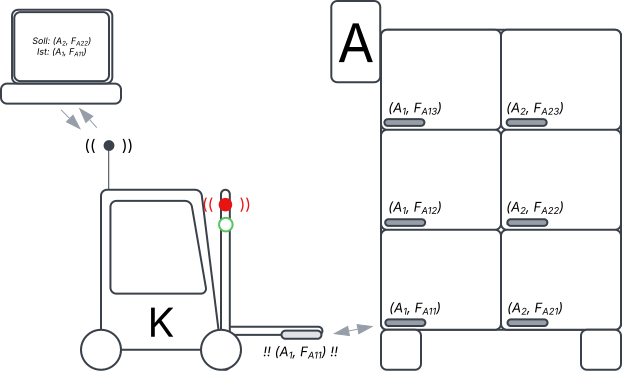
\includegraphics[scale=0.6]{aufgabe 2/img/auftrag.svg}
    \caption{Skizzenhafte Darstellung eines Fahrauftrages. Es ist das Staplerfahrzeug $K$ mit dem Fahrauftrag $(A_2, F_{A22})$ dargestellt sowie das Regal $A$, das aus zwei Regalpositionen mit jeweils drei Fächern (Palettenpositionen) besteht.  (Quelle: eigene)}
    \label{fig:auftrag}
\end{figure}